\PassOptionsToPackage{dvipsnames,table}{xcolor}
\documentclass[10pt]{beamer}
\usepackage{Cours}

\begin{document}



\newcounter{numchap}
\setcounter{numchap}{1}
\newcounter{numframe}
\setcounter{numframe}{0}
\newcommand{\mframe}[1]{\frametitle{#1} \addtocounter{numframe}{1}}
\newcommand{\cnum}{\fbox{\textcolor{yellow}{\textbf{C\thenumchap}}}~}
\newcommand{\makess}[1]{\section{#1} \label{ss\thesection}}
\newcommand{\stitle}{\textcolor{yellow}{\textbf{\thesection. \nameref{ss\thesection}}}}

\definecolor{codebg}{gray}{0.90}
\definecolor{grispale}{gray}{0.95}
\definecolor{fluo}{rgb}{1,0.96,0.62}
\newminted[langageC]{c}{linenos=true,escapeinside=||,highlightcolor=fluo,tabsize=2,breaklines=true}
\newminted[codepython]{python}{linenos=true,escapeinside=||,highlightcolor=fluo,tabsize=2,breaklines=true}
% Inclusion complète (ou partiel en indiquant premiere et dernière ligne) d'un fichier C
\newcommand{\inputC}[3]{\begin{mdframed}[backgroundcolor=codebg] \inputminted[breaklines=true,fontsize=#3,linenos=true,highlightcolor=fluo,tabsize=2,highlightlines={#2}]{c}{#1} \end{mdframed}}
\newcommand{\inputpartC}[5]{\begin{mdframed}[backgroundcolor=codebg] \inputminted[breaklines=true,fontsize=#3,linenos=true,highlightcolor=fluo,tabsize=2,highlightlines={#2},firstline=#4,lastline=#5,firstnumber=1]{c}{#1} \end{mdframed}}
\newcommand{\inputpython}[3]{\begin{mdframed}[backgroundcolor=codebg] \inputminted[breaklines=true,fontsize=#3,linenos=true,highlightcolor=fluo,tabsize=2,highlightlines={#2}]{python}{#1} \end{mdframed}}
\newcommand{\inputpartOCaml}[5]{\begin{mdframed}[backgroundcolor=codebg] \inputminted[breaklines=true,fontsize=#3,linenos=true,highlightcolor=fluo,tabsize=2,highlightlines={#2},firstline=#4,lastline=#5,firstnumber=1]{OCaml}{#1} \end{mdframed}}
\BeforeBeginEnvironment{minted}{\begin{mdframed}[backgroundcolor=codebg]}
\AfterEndEnvironment{minted}{\end{mdframed}}
\newcommand{\kw}[1]{\textcolor{blue}{\tt #1}}

\newtcolorbox{rcadre}[4]{halign=center,colback={#1},colframe={#2},width={#3cm},height={#4cm},valign=center,boxrule=1pt,left=0pt,right=0pt}
\newtcolorbox{cadre}[4]{halign=center,colback={#1},colframe={#2},arc=0mm,width={#3cm},height={#4cm},valign=center,boxrule=1pt,left=0pt,right=0pt}
\newcommand{\myem}[1]{\colorbox{fluo}{#1}}
\mdfsetup{skipabove=1pt,skipbelow=-2pt}



% Noeud dans un cadre pour les arbres
\newcommand{\noeud}[2]{\Tr{\fbox{\textcolor{#1}{\tt #2}}}}

\newcommand{\htmlmode}{\lstset{language=html,numbers=left, tabsize=4, frame=single, breaklines=true, keywordstyle=\ttfamily, basicstyle=\small,
   numberstyle=\tiny\ttfamily, framexleftmargin=0mm, backgroundcolor=\color{grispale}, xleftmargin=12mm,showstringspaces=false}}
\newcommand{\pythonmode}{\lstset{
   language=python,
   linewidth=\linewidth,
   numbers=left,
   tabsize=4,
   frame=single,
   breaklines=true,
   keywordstyle=\ttfamily\color{blue},
   basicstyle=\small,
   numberstyle=\tiny\ttfamily,
   framexleftmargin=-2mm,
   numbersep=-0.5mm,
   backgroundcolor=\color{codebg},
   xleftmargin=-1mm, 
   showstringspaces=false,
   commentstyle=\color{gray},
   stringstyle=\color{OliveGreen},
   emph={turtle,Screen,Turtle},
   emphstyle=\color{RawSienna},
   morekeywords={setheading,goto,backward,forward,left,right,pendown,penup,pensize,color,speed,hideturtle,showturtle,forward}}
   }
   \newcommand{\Cmode}{\lstset{
      language=[ANSI]C,
      linewidth=\linewidth,
      numbers=left,
      tabsize=4,
      frame=single,
      breaklines=true,
      keywordstyle=\ttfamily\color{blue},
      basicstyle=\small,
      numberstyle=\tiny\ttfamily,
      framexleftmargin=0mm,
      numbersep=2mm,
      backgroundcolor=\color{codebg},
      xleftmargin=0mm, 
      showstringspaces=false,
      commentstyle=\color{gray},
      stringstyle=\color{OliveGreen},
      emphstyle=\color{RawSienna},
      escapechar=\|,
      morekeywords={}}
      }
\newcommand{\bashmode}{\lstset{language=bash,numbers=left, tabsize=2, frame=single, breaklines=true, basicstyle=\ttfamily,
   numberstyle=\tiny\ttfamily, framexleftmargin=0mm, backgroundcolor=\color{grispale}, xleftmargin=12mm, showstringspaces=false}}
\newcommand{\exomode}{\lstset{language=python,numbers=left, tabsize=2, frame=single, breaklines=true, basicstyle=\ttfamily,
   numberstyle=\tiny\ttfamily, framexleftmargin=13mm, xleftmargin=12mm, basicstyle=\small, showstringspaces=false}}
   
   
  
%tei pour placer les images
%tei{nom de l’image}{échelle de l’image}{sens}{texte a positionner}
%sens ="1" (droite) ou "2" (gauche)
\newlength{\ltxt}
\newcommand{\tei}[4]{
\setlength{\ltxt}{\linewidth}
\setbox0=\hbox{\includegraphics[scale=#2]{#1}}
\addtolength{\ltxt}{-\wd0}
\addtolength{\ltxt}{-10pt}
\ifthenelse{\equal{#3}{1}}{
\begin{minipage}{\wd0}
\includegraphics[scale=#2]{#1}
\end{minipage}
\hfill
\begin{minipage}{\ltxt}
#4
\end{minipage}
}{
\begin{minipage}{\ltxt}
#4
\end{minipage}
\hfill
\begin{minipage}{\wd0}
\includegraphics[scale=#2]{#1}
\end{minipage}
}
}

%Juxtaposition d'une image pspciture et de texte 
%#1: = code pstricks de l'image
%#2: largeur de l'image
%#3: hauteur de l'image
%#4: Texte à écrire
\newcommand{\ptp}[4]{
\setlength{\ltxt}{\linewidth}
\addtolength{\ltxt}{-#2 cm}
\addtolength{\ltxt}{-0.1 cm}
\begin{minipage}[b][#3 cm][t]{\ltxt}
#4
\end{minipage}\hfill
\begin{minipage}[b][#3 cm][c]{#2 cm}
#1
\end{minipage}\par
}



%Macros pour les graphiques
\psset{linewidth=0.5\pslinewidth,PointSymbol=x}
\setlength{\fboxrule}{0.5pt}
\newcounter{tempangle}

%Marque la longueur du segment d'extrémité  #1 et  #2 avec la valeur #3, #4 est la distance par rapport au segment (en %age de la valeur de celui ci) et #5 l'orientation du marquage : +90 ou -90
\newcommand{\afflong}[5]{
\pstRotation[RotAngle=#4,PointSymbol=none,PointName=none]{#1}{#2}[X] 
\pstHomO[PointSymbol=none,PointName=none,HomCoef=#5]{#1}{X}[Y]
\pstTranslation[PointSymbol=none,PointName=none]{#1}{#2}{Y}[Z]
 \ncline{|<->|,linewidth=0.25\pslinewidth}{Y}{Z} \ncput*[nrot=:U]{\footnotesize{#3}}
}
\newcommand{\afflongb}[3]{
\ncline{|<->|,linewidth=0}{#1}{#2} \naput*[nrot=:U]{\footnotesize{#3}}
}

%Construis le point #4 situé à #2 cm du point #1 avant un angle #3 par rapport à l'horizontale. #5 = liste de paramètre
\newcommand{\lsegment}[5]{\pstGeonode[PointSymbol=none,PointName=none](0,0){O'}(#2,0){I'} \pstTranslation[PointSymbol=none,PointName=none]{O'}{I'}{#1}[J'] \pstRotation[RotAngle=#3,PointSymbol=x,#5]{#1}{J'}[#4]}
\newcommand{\tsegment}[5]{\pstGeonode[PointSymbol=none,PointName=none](0,0){O'}(#2,0){I'} \pstTranslation[PointSymbol=none,PointName=none]{O'}{I'}{#1}[J'] \pstRotation[RotAngle=#3,PointSymbol=x,#5]{#1}{J'}[#4] \pstLineAB{#4}{#1}}

%Construis le point #4 situé à #3 cm du point #1 et faisant un angle de  90° avec la droite (#1,#2) #5 = liste de paramètre
\newcommand{\psegment}[5]{
\pstGeonode[PointSymbol=none,PointName=none](0,0){O'}(#3,0){I'}
 \pstTranslation[PointSymbol=none,PointName=none]{O'}{I'}{#1}[J']
 \pstInterLC[PointSymbol=none,PointName=none]{#1}{#2}{#1}{J'}{M1}{M2} \pstRotation[RotAngle=-90,PointSymbol=x,#5]{#1}{M1}[#4]
  }
  
%Construis le point #4 situé à #3 cm du point #1 et faisant un angle de  #5° avec la droite (#1,#2) #6 = liste de paramètre
\newcommand{\mlogo}[6]{
\pstGeonode[PointSymbol=none,PointName=none](0,0){O'}(#3,0){I'}
 \pstTranslation[PointSymbol=none,PointName=none]{O'}{I'}{#1}[J']
 \pstInterLC[PointSymbol=none,PointName=none]{#1}{#2}{#1}{J'}{M1}{M2} \pstRotation[RotAngle=#5,PointSymbol=x,#6]{#1}{M2}[#4]
  }

% Construis un triangle avec #1=liste des 3 sommets séparés par des virgules, #2=liste des 3 longueurs séparés par des virgules, #3 et #4 : paramètre d'affichage des 2e et 3 points et #5 : inclinaison par rapport à l'horizontale
%autre macro identique mais sans tracer les segments joignant les sommets
\noexpandarg
\newcommand{\Triangleccc}[5]{
\StrBefore{#1}{,}[\pointA]
\StrBetween[1,2]{#1}{,}{,}[\pointB]
\StrBehind[2]{#1}{,}[\pointC]
\StrBefore{#2}{,}[\coteA]
\StrBetween[1,2]{#2}{,}{,}[\coteB]
\StrBehind[2]{#2}{,}[\coteC]
\tsegment{\pointA}{\coteA}{#5}{\pointB}{#3} 
\lsegment{\pointA}{\coteB}{0}{Z1}{PointSymbol=none, PointName=none}
\lsegment{\pointB}{\coteC}{0}{Z2}{PointSymbol=none, PointName=none}
\pstInterCC{\pointA}{Z1}{\pointB}{Z2}{\pointC}{Z3} 
\pstLineAB{\pointA}{\pointC} \pstLineAB{\pointB}{\pointC}
\pstSymO[PointName=\pointC,#4]{C}{C}[C]
}
\noexpandarg
\newcommand{\TrianglecccP}[5]{
\StrBefore{#1}{,}[\pointA]
\StrBetween[1,2]{#1}{,}{,}[\pointB]
\StrBehind[2]{#1}{,}[\pointC]
\StrBefore{#2}{,}[\coteA]
\StrBetween[1,2]{#2}{,}{,}[\coteB]
\StrBehind[2]{#2}{,}[\coteC]
\tsegment{\pointA}{\coteA}{#5}{\pointB}{#3} 
\lsegment{\pointA}{\coteB}{0}{Z1}{PointSymbol=none, PointName=none}
\lsegment{\pointB}{\coteC}{0}{Z2}{PointSymbol=none, PointName=none}
\pstInterCC[PointNameB=none,PointSymbolB=none,#4]{\pointA}{Z1}{\pointB}{Z2}{\pointC}{Z1} 
}


% Construis un triangle avec #1=liste des 3 sommets séparés par des virgules, #2=liste formée de 2 longueurs et d'un angle séparés par des virgules, #3 et #4 : paramètre d'affichage des 2e et 3 points et #5 : inclinaison par rapport à l'horizontale
%autre macro identique mais sans tracer les segments joignant les sommets
\newcommand{\Trianglecca}[5]{
\StrBefore{#1}{,}[\pointA]
\StrBetween[1,2]{#1}{,}{,}[\pointB]
\StrBehind[2]{#1}{,}[\pointC]
\StrBefore{#2}{,}[\coteA]
\StrBetween[1,2]{#2}{,}{,}[\coteB]
\StrBehind[2]{#2}{,}[\angleA]
\tsegment{\pointA}{\coteA}{#5}{\pointB}{#3} 
\setcounter{tempangle}{#5}
\addtocounter{tempangle}{\angleA}
\tsegment{\pointA}{\coteB}{\thetempangle}{\pointC}{#4}
\pstLineAB{\pointB}{\pointC}
}
\newcommand{\TriangleccaP}[5]{
\StrBefore{#1}{,}[\pointA]
\StrBetween[1,2]{#1}{,}{,}[\pointB]
\StrBehind[2]{#1}{,}[\pointC]
\StrBefore{#2}{,}[\coteA]
\StrBetween[1,2]{#2}{,}{,}[\coteB]
\StrBehind[2]{#2}{,}[\angleA]
\lsegment{\pointA}{\coteA}{#5}{\pointB}{#3} 
\setcounter{tempangle}{#5}
\addtocounter{tempangle}{\angleA}
\lsegment{\pointA}{\coteB}{\thetempangle}{\pointC}{#4}
}

% Construis un triangle avec #1=liste des 3 sommets séparés par des virgules, #2=liste formée de 1 longueurs et de deux angle séparés par des virgules, #3 et #4 : paramètre d'affichage des 2e et 3 points et #5 : inclinaison par rapport à l'horizontale
%autre macro identique mais sans tracer les segments joignant les sommets
\newcommand{\Trianglecaa}[5]{
\StrBefore{#1}{,}[\pointA]
\StrBetween[1,2]{#1}{,}{,}[\pointB]
\StrBehind[2]{#1}{,}[\pointC]
\StrBefore{#2}{,}[\coteA]
\StrBetween[1,2]{#2}{,}{,}[\angleA]
\StrBehind[2]{#2}{,}[\angleB]
\tsegment{\pointA}{\coteA}{#5}{\pointB}{#3} 
\setcounter{tempangle}{#5}
\addtocounter{tempangle}{\angleA}
\lsegment{\pointA}{1}{\thetempangle}{Z1}{PointSymbol=none, PointName=none}
\setcounter{tempangle}{#5}
\addtocounter{tempangle}{180}
\addtocounter{tempangle}{-\angleB}
\lsegment{\pointB}{1}{\thetempangle}{Z2}{PointSymbol=none, PointName=none}
\pstInterLL[#4]{\pointA}{Z1}{\pointB}{Z2}{\pointC}
\pstLineAB{\pointA}{\pointC}
\pstLineAB{\pointB}{\pointC}
}
\newcommand{\TrianglecaaP}[5]{
\StrBefore{#1}{,}[\pointA]
\StrBetween[1,2]{#1}{,}{,}[\pointB]
\StrBehind[2]{#1}{,}[\pointC]
\StrBefore{#2}{,}[\coteA]
\StrBetween[1,2]{#2}{,}{,}[\angleA]
\StrBehind[2]{#2}{,}[\angleB]
\lsegment{\pointA}{\coteA}{#5}{\pointB}{#3} 
\setcounter{tempangle}{#5}
\addtocounter{tempangle}{\angleA}
\lsegment{\pointA}{1}{\thetempangle}{Z1}{PointSymbol=none, PointName=none}
\setcounter{tempangle}{#5}
\addtocounter{tempangle}{180}
\addtocounter{tempangle}{-\angleB}
\lsegment{\pointB}{1}{\thetempangle}{Z2}{PointSymbol=none, PointName=none}
\pstInterLL[#4]{\pointA}{Z1}{\pointB}{Z2}{\pointC}
}

%Construction d'un cercle de centre #1 et de rayon #2 (en cm)
\newcommand{\Cercle}[2]{
\lsegment{#1}{#2}{0}{Z1}{PointSymbol=none, PointName=none}
\pstCircleOA{#1}{Z1}
}

%construction d'un parallélogramme #1 = liste des sommets, #2 = liste contenant les longueurs de 2 côtés consécutifs et leurs angles;  #3, #4 et #5 : paramètre d'affichage des sommets #6 inclinaison par rapport à l'horizontale 
% meme macro sans le tracé des segements
\newcommand{\Para}[6]{
\StrBefore{#1}{,}[\pointA]
\StrBetween[1,2]{#1}{,}{,}[\pointB]
\StrBetween[2,3]{#1}{,}{,}[\pointC]
\StrBehind[3]{#1}{,}[\pointD]
\StrBefore{#2}{,}[\longueur]
\StrBetween[1,2]{#2}{,}{,}[\largeur]
\StrBehind[2]{#2}{,}[\angle]
\tsegment{\pointA}{\longueur}{#6}{\pointB}{#3} 
\setcounter{tempangle}{#6}
\addtocounter{tempangle}{\angle}
\tsegment{\pointA}{\largeur}{\thetempangle}{\pointD}{#5}
\pstMiddleAB[PointName=none,PointSymbol=none]{\pointB}{\pointD}{Z1}
\pstSymO[#4]{Z1}{\pointA}[\pointC]
\pstLineAB{\pointB}{\pointC}
\pstLineAB{\pointC}{\pointD}
}
\newcommand{\ParaP}[6]{
\StrBefore{#1}{,}[\pointA]
\StrBetween[1,2]{#1}{,}{,}[\pointB]
\StrBetween[2,3]{#1}{,}{,}[\pointC]
\StrBehind[3]{#1}{,}[\pointD]
\StrBefore{#2}{,}[\longueur]
\StrBetween[1,2]{#2}{,}{,}[\largeur]
\StrBehind[2]{#2}{,}[\angle]
\lsegment{\pointA}{\longueur}{#6}{\pointB}{#3} 
\setcounter{tempangle}{#6}
\addtocounter{tempangle}{\angle}
\lsegment{\pointA}{\largeur}{\thetempangle}{\pointD}{#5}
\pstMiddleAB[PointName=none,PointSymbol=none]{\pointB}{\pointD}{Z1}
\pstSymO[#4]{Z1}{\pointA}[\pointC]
}


%construction d'un cerf-volant #1 = liste des sommets, #2 = liste contenant les longueurs de 2 côtés consécutifs et leurs angles;  #3, #4 et #5 : paramètre d'affichage des sommets #6 inclinaison par rapport à l'horizontale 
% meme macro sans le tracé des segements
\newcommand{\CerfVolant}[6]{
\StrBefore{#1}{,}[\pointA]
\StrBetween[1,2]{#1}{,}{,}[\pointB]
\StrBetween[2,3]{#1}{,}{,}[\pointC]
\StrBehind[3]{#1}{,}[\pointD]
\StrBefore{#2}{,}[\longueur]
\StrBetween[1,2]{#2}{,}{,}[\largeur]
\StrBehind[2]{#2}{,}[\angle]
\tsegment{\pointA}{\longueur}{#6}{\pointB}{#3} 
\setcounter{tempangle}{#6}
\addtocounter{tempangle}{\angle}
\tsegment{\pointA}{\largeur}{\thetempangle}{\pointD}{#5}
\pstOrtSym[#4]{\pointB}{\pointD}{\pointA}[\pointC]
\pstLineAB{\pointB}{\pointC}
\pstLineAB{\pointC}{\pointD}
}

%construction d'un quadrilatère quelconque #1 = liste des sommets, #2 = liste contenant les longueurs des 4 côtés et l'angle entre 2 cotés consécutifs  #3, #4 et #5 : paramètre d'affichage des sommets #6 inclinaison par rapport à l'horizontale 
% meme macro sans le tracé des segements
\newcommand{\Quadri}[6]{
\StrBefore{#1}{,}[\pointA]
\StrBetween[1,2]{#1}{,}{,}[\pointB]
\StrBetween[2,3]{#1}{,}{,}[\pointC]
\StrBehind[3]{#1}{,}[\pointD]
\StrBefore{#2}{,}[\coteA]
\StrBetween[1,2]{#2}{,}{,}[\coteB]
\StrBetween[2,3]{#2}{,}{,}[\coteC]
\StrBetween[3,4]{#2}{,}{,}[\coteD]
\StrBehind[4]{#2}{,}[\angle]
\tsegment{\pointA}{\coteA}{#6}{\pointB}{#3} 
\setcounter{tempangle}{#6}
\addtocounter{tempangle}{\angle}
\tsegment{\pointA}{\coteD}{\thetempangle}{\pointD}{#5}
\lsegment{\pointB}{\coteB}{0}{Z1}{PointSymbol=none, PointName=none}
\lsegment{\pointD}{\coteC}{0}{Z2}{PointSymbol=none, PointName=none}
\pstInterCC[PointNameA=none,PointSymbolA=none,#4]{\pointB}{Z1}{\pointD}{Z2}{Z3}{\pointC} 
\pstLineAB{\pointB}{\pointC}
\pstLineAB{\pointC}{\pointD}
}


% Définition des colonnes centrées ou à droite pour tabularx
\newcolumntype{Y}{>{\centering\arraybackslash}X}
\newcolumntype{Z}{>{\flushright\arraybackslash}X}

%Les pointillés à remplir par les élèves
\newcommand{\po}[1]{\makebox[#1 cm]{\dotfill}}
\newcommand{\lpo}[1][3]{%
\multido{}{#1}{\makebox[\linewidth]{\dotfill}
}}

%Liste des pictogrammes utilisés sur la fiche d'exercice ou d'activités
\newcommand{\bombe}{\faBomb}
\newcommand{\livre}{\faBook}
\newcommand{\calculatrice}{\faCalculator}
\newcommand{\oral}{\faCommentO}
\newcommand{\surfeuille}{\faEdit}
\newcommand{\ordinateur}{\faLaptop}
\newcommand{\ordi}{\faDesktop}
\newcommand{\ciseaux}{\faScissors}
\newcommand{\danger}{\faExclamationTriangle}
\newcommand{\out}{\faSignOut}
\newcommand{\cadeau}{\faGift}
\newcommand{\flash}{\faBolt}
\newcommand{\lumiere}{\faLightbulb}
\newcommand{\compas}{\dsmathematical}
\newcommand{\calcullitteral}{\faTimesCircleO}
\newcommand{\raisonnement}{\faCogs}
\newcommand{\recherche}{\faSearch}
\newcommand{\rappel}{\faHistory}
\newcommand{\video}{\faFilm}
\newcommand{\capacite}{\faPuzzlePiece}
\newcommand{\aide}{\faLifeRing}
\newcommand{\loin}{\faExternalLink}
\newcommand{\groupe}{\faUsers}
\newcommand{\bac}{\faGraduationCap}
\newcommand{\histoire}{\faUniversity}
\newcommand{\coeur}{\faSave}
\newcommand{\python}{\faPython}
\newcommand{\os}{\faMicrochip}
\newcommand{\rd}{\faCubes}
\newcommand{\data}{\faColumns}
\newcommand{\web}{\faCode}
\newcommand{\prog}{\faFile}
\newcommand{\algo}{\faCogs}
\newcommand{\important}{\faExclamationCircle}
\newcommand{\maths}{\faTimesCircle}
% Traitement des données en tables
\newcommand{\tables}{\faColumns}
% Types construits
\newcommand{\construits}{\faCubes}
% Type et valeurs de base
\newcommand{\debase}{{\footnotesize \faCube}}
% Systèmes d'exploitation
\newcommand{\linux}{\faLinux}
\newcommand{\sd}{\faProjectDiagram}
\newcommand{\bd}{\faDatabase}

%Les ensembles de nombres
\renewcommand{\N}{\mathbb{N}}
\newcommand{\D}{\mathbb{D}}
\newcommand{\Z}{\mathbb{Z}}
\newcommand{\Q}{\mathbb{Q}}
\newcommand{\R}{\mathbb{R}}
\newcommand{\C}{\mathbb{C}}

%Ecriture des vecteurs
\newcommand{\vect}[1]{\vbox{\halign{##\cr 
  \tiny\rightarrowfill\cr\noalign{\nointerlineskip\vskip1pt} 
  $#1\mskip2mu$\cr}}}


%Compteur activités/exos et question et mise en forme titre et questions
\newcounter{numact}
\setcounter{numact}{1}
\newcounter{numseance}
\setcounter{numseance}{1}
\newcounter{numexo}
\setcounter{numexo}{0}
\newcounter{numprojet}
\setcounter{numprojet}{0}
\newcounter{numquestion}
\newcommand{\espace}[1]{\rule[-1ex]{0pt}{#1 cm}}
\newcommand{\Quest}[3]{
\addtocounter{numquestion}{1}
\begin{tabularx}{\textwidth}{X|m{1cm}|}
\cline{2-2}
\textbf{\sffamily{\alph{numquestion})}} #1 & \dots / #2 \\
\hline 
\multicolumn{2}{|l|}{\espace{#3}} \\
\hline
\end{tabularx}
}
\newcommand{\QuestR}[3]{
\addtocounter{numquestion}{1}
\begin{tabularx}{\textwidth}{X|m{1cm}|}
\cline{2-2}
\textbf{\sffamily{\alph{numquestion})}} #1 & \dots / #2 \\
\hline 
\multicolumn{2}{|l|}{\cor{#3}} \\
\hline
\end{tabularx}
}
\newcommand{\Pre}{{\sc nsi} 1\textsuperscript{e}}
\newcommand{\Term}{{\sc nsi} Terminale}
\newcommand{\Sec}{2\textsuperscript{e}}
\newcommand{\Exo}[2]{ \addtocounter{numexo}{1} \ding{113} \textbf{\sffamily{Exercice \thenumexo}} : \textit{#1} \hfill #2  \setcounter{numquestion}{0}}
\newcommand{\Projet}[1]{ \addtocounter{numprojet}{1} \ding{118} \textbf{\sffamily{Projet \thenumprojet}} : \textit{#1}}
\newcommand{\ExoD}[2]{ \addtocounter{numexo}{1} \ding{113} \textbf{\sffamily{Exercice \thenumexo}}  \textit{(#1 pts)} \hfill #2  \setcounter{numquestion}{0}}
\newcommand{\ExoB}[2]{ \addtocounter{numexo}{1} \ding{113} \textbf{\sffamily{Exercice \thenumexo}}  \textit{(Bonus de +#1 pts maximum)} \hfill #2  \setcounter{numquestion}{0}}
\newcommand{\Act}[2]{ \ding{113} \textbf{\sffamily{Activité \thenumact}} : \textit{#1} \hfill #2  \addtocounter{numact}{1} \setcounter{numquestion}{0}}
\newcommand{\Seance}{ \rule{1.5cm}{0.5pt}\raisebox{-3pt}{\framebox[4cm]{\textbf{\sffamily{Séance \thenumseance}}}}\hrulefill  \\
  \addtocounter{numseance}{1}}
\newcommand{\Acti}[2]{ {\footnotesize \ding{117}} \textbf{\sffamily{Activité \thenumact}} : \textit{#1} \hfill #2  \addtocounter{numact}{1} \setcounter{numquestion}{0}}
\newcommand{\titre}[1]{\begin{Large}\textbf{\ding{118}}\end{Large} \begin{large}\textbf{ #1}\end{large} \vspace{0.2cm}}
\newcommand{\QListe}[1][0]{
\ifthenelse{#1=0}
{\begin{enumerate}[partopsep=0pt,topsep=0pt,parsep=0pt,itemsep=0pt,label=\textbf{\sffamily{\arabic*.}},series=question]}
{\begin{enumerate}[resume*=question]}}
\newcommand{\SQListe}[1][0]{
\ifthenelse{#1=0}
{\begin{enumerate}[partopsep=0pt,topsep=0pt,parsep=0pt,itemsep=0pt,label=\textbf{\sffamily{\alph*)}},series=squestion]}
{\begin{enumerate}[resume*=squestion]}}
\newcommand{\SQListeL}[1][0]{
\ifthenelse{#1=0}
{\begin{enumerate*}[partopsep=0pt,topsep=0pt,parsep=0pt,itemsep=0pt,label=\textbf{\sffamily{\alph*)}},series=squestion]}
{\begin{enumerate*}[resume*=squestion]}}
\newcommand{\FinListe}{\end{enumerate}}
\newcommand{\FinListeL}{\end{enumerate*}}

%Mise en forme de la correction
\newcommand{\cor}[1]{\par \textcolor{OliveGreen}{#1}}
\newcommand{\br}[1]{\cor{\textbf{#1}}}
\newcommand{\tcor}[1]{\begin{tcolorbox}[width=0.92\textwidth,colback={white},colbacktitle=white,coltitle=OliveGreen,colframe=green!75!black,boxrule=0.2mm]   
\cor{#1}
\end{tcolorbox}
}
\newcommand{\rc}[1]{\textcolor{OliveGreen}{#1}}
\newcommand{\pmc}[1]{\textcolor{blue}{\tt #1}}
\newcommand{\tmc}[1]{\textcolor{RawSienna}{\tt #1}}


%Référence aux exercices par leur numéro
\newcommand{\refexo}[1]{
\refstepcounter{numexo}
\addtocounter{numexo}{-1}
\label{#1}}

%Séparation entre deux activités
\newcommand{\separateur}{\begin{center}
\rule{1.5cm}{0.5pt}\raisebox{-3pt}{\ding{117}}\rule{1.5cm}{0.5pt}  \vspace{0.2cm}
\end{center}}

%Entête et pied de page
\newcommand{\snt}[1]{\lhead{\textbf{SNT -- La photographie numérique} \rhead{\textit{Lycée Nord}}}}
\newcommand{\Activites}[2]{\lhead{\textbf{{\sc #1}}}
\rhead{Activités -- \textbf{#2}}
\cfoot{}}
\newcommand{\Exos}[2]{\lhead{\textbf{Fiche d'exercices: {\sc #1}}}
\rhead{Niveau: \textbf{#2}}
\cfoot{}}
\newcommand{\Devoir}[2]{\lhead{\textbf{Devoir de mathématiques : {\sc #1}}}
\rhead{\textbf{#2}} \setlength{\fboxsep}{8pt}
\begin{center}
%Titre de la fiche
\fbox{\parbox[b][1cm][t]{0.3\textwidth}{Nom : \hfill \po{3} \par \vfill Prénom : \hfill \po{3}} } \hfill 
\fbox{\parbox[b][1cm][t]{0.6\textwidth}{Note : \po{1} / 20} }
\end{center} \cfoot{}}

%Devoir programmation en NSI (pas à rendre sur papier)
\newcommand{\PNSI}[2]{\lhead{\textbf{Devoir de {\sc nsi} : \textsf{ #1}}}
\rhead{\textbf{#2}} \setlength{\fboxsep}{8pt}
\begin{tcolorbox}[title=\textcolor{black}{\danger\; A lire attentivement},colbacktitle=lightgray]
{\begin{enumerate}
\item Rendre tous vous programmes en les envoyant par mail à l'adresse {\tt fnativel2@ac-reunion.fr}, en précisant bien dans le sujet vos noms et prénoms
\item Un programme qui fonctionne mal ou pas du tout peut rapporter des points
\item Les bonnes pratiques de programmation (clarté et lisiblité du code) rapportent des points
\end{enumerate}
}
\end{tcolorbox}
 \cfoot{}}


%Devoir de NSI
\newcommand{\DNSI}[2]{\lhead{\textbf{Devoir de {\sc nsi} : \textsf{ #1}}}
\rhead{\textbf{#2}} \setlength{\fboxsep}{8pt}
\begin{center}
%Titre de la fiche
\fbox{\parbox[b][1cm][t]{0.3\textwidth}{Nom : \hfill \po{3} \par \vfill Prénom : \hfill \po{3}} } \hfill 
\fbox{\parbox[b][1cm][t]{0.6\textwidth}{Note : \po{1} / 10} }
\end{center} \cfoot{}}

\newcommand{\DevoirNSI}[2]{\lhead{\textbf{Devoir de {\sc nsi} : {\sc #1}}}
\rhead{\textbf{#2}} \setlength{\fboxsep}{8pt}
\cfoot{}}

%La définition de la commande QCM pour auto-multiple-choice
%En premier argument le sujet du qcm, deuxième argument : la classe, 3e : la durée prévue et #4 : présence ou non de questions avec plusieurs bonnes réponses
\newcommand{\QCM}[4]{
{\large \textbf{\ding{52} QCM : #1}} -- Durée : \textbf{#3 min} \hfill {\large Note : \dots/10} 
\hrule \vspace{0.1cm}\namefield{}
Nom :  \textbf{\textbf{\nom{}}} \qquad \qquad Prénom :  \textbf{\prenom{}}  \hfill Classe: \textbf{#2}
\vspace{0.2cm}
\hrule  
\begin{itemize}[itemsep=0pt]
\item[-] \textit{Une bonne réponse vaut un point, une absence de réponse n'enlève pas de point. }
\item[\danger] \textit{Une mauvaise réponse enlève un point.}
\ifthenelse{#4=1}{\item[-] \textit{Les questions marquées du symbole \multiSymbole{} peuvent avoir plusieurs bonnes réponses possibles.}}{}
\end{itemize}
}
\newcommand{\DevoirC}[2]{
\renewcommand{\footrulewidth}{0.5pt}
\lhead{\textbf{Devoir de mathématiques : {\sc #1}}}
\rhead{\textbf{#2}} \setlength{\fboxsep}{8pt}
\fbox{\parbox[b][0.4cm][t]{0.955\textwidth}{Nom : \po{5} \hfill Prénom : \po{5} \hfill Classe: \textbf{1}\textsuperscript{$\dots$}} } 
\rfoot{\thepage} \cfoot{} \lfoot{Lycée Nord}}
\newcommand{\DevoirInfo}[2]{\lhead{\textbf{Evaluation : {\sc #1}}}
\rhead{\textbf{#2}} \setlength{\fboxsep}{8pt}
 \cfoot{}}
\newcommand{\DM}[2]{\lhead{\textbf{Devoir maison à rendre le #1}} \rhead{\textbf{#2}}}

%Macros permettant l'affichage des touches de la calculatrice
%Touches classiques : #1 = 0 fond blanc pour les nombres et #1= 1gris pour les opérations et entrer, second paramètre=contenu
%Si #2=1 touche arrondi avec fond gris
\newcommand{\TCalc}[2]{
\setlength{\fboxsep}{0.1pt}
\ifthenelse{#1=0}
{\psframebox[fillstyle=solid, fillcolor=white]{\parbox[c][0.25cm][c]{0.6cm}{\centering #2}}}
{\ifthenelse{#1=1}
{\psframebox[fillstyle=solid, fillcolor=lightgray]{\parbox[c][0.25cm][c]{0.6cm}{\centering #2}}}
{\psframebox[framearc=.5,fillstyle=solid, fillcolor=white]{\parbox[c][0.25cm][c]{0.6cm}{\centering #2}}}
}}
\newcommand{\Talpha}{\psdblframebox[fillstyle=solid, fillcolor=white]{\hspace{-0.05cm}\parbox[c][0.25cm][c]{0.65cm}{\centering \scriptsize{alpha}}} \;}
\newcommand{\Tsec}{\psdblframebox[fillstyle=solid, fillcolor=white]{\parbox[c][0.25cm][c]{0.6cm}{\centering \scriptsize 2nde}} \;}
\newcommand{\Tfx}{\psdblframebox[fillstyle=solid, fillcolor=white]{\parbox[c][0.25cm][c]{0.6cm}{\centering \scriptsize $f(x)$}} \;}
\newcommand{\Tvar}{\psframebox[framearc=.5,fillstyle=solid, fillcolor=white]{\hspace{-0.22cm} \parbox[c][0.25cm][c]{0.82cm}{$\scriptscriptstyle{X,T,\theta,n}$}}}
\newcommand{\Tgraphe}{\psdblframebox[fillstyle=solid, fillcolor=white]{\hspace{-0.08cm}\parbox[c][0.25cm][c]{0.68cm}{\centering \tiny{graphe}}} \;}
\newcommand{\Tfen}{\psdblframebox[fillstyle=solid, fillcolor=white]{\hspace{-0.08cm}\parbox[c][0.25cm][c]{0.68cm}{\centering \tiny{fenêtre}}} \;}
\newcommand{\Ttrace}{\psdblframebox[fillstyle=solid, fillcolor=white]{\parbox[c][0.25cm][c]{0.6cm}{\centering \scriptsize{trace}}} \;}

% Macroi pour l'affichage  d'un entier n dans  une base b
\newcommand{\base}[2]{ \overline{#1}^{#2}}
% Intervalle d'entiers
\newcommand{\intN}[2]{\llbracket #1; #2 \rrbracket}}

% Numéro et titre de chapitre
\setcounter{numchap}{15}
\newcommand{\Ctitle}{\cnum {Décomposition en sous problèmes}}
\newcommand{\SPATH}{/home/fenarius/Travail/Cours/cpge-info/docs/mp2i/files/C\thenumchap/}

\makess{Introduction}
\begin{frame}{\Ctitle}{\stitle}
	\begin{block}{Principe général}
		Pour résoudre un problème donné, une stratégie peut-être de se ramener à un ou plusieurs sous problèmes de \textit{même type} mais \textit{plus petit}. En notant $P(n)$, un problème de taille $n$, la résolution de $P_n$ conduit à la résolution de $k$ problèmes de tailles $P(\frac{n}{p})$. Un fois ces problèmes résolus, leurs solutions sont combinées afin de former celle du problème initial. \\
		\smallskip
		\onslide<2->{On distingue :}
		\begin{itemize}
			\item<3-> la méthode \textcolor{blue}{diviser pour régner}, dans laquelle les sous-problèmes sont indépendants
			\item<4-> la méthode de \textcolor{blue}{programmation dynamique} dans laquelle, certains sous problèmes se chevauchent.
		\end{itemize}
	\end{block}
\end{frame}

\makess{Diviser pour regner}
\begin{frame}{\Ctitle}{\stitle}
	\begin{exampleblock}{Exemple introductif}
		Le tri fusion est l'exemple typique d'une résolution par la méthode diviser pour régner. En effet, pour trier une liste $l$ de taille $n$,
		\begin{itemize}
			\item<2-> \textcolor{blue}{Diviser} : on sépare $l$ en deux moitiés (à une unité près) $l_1$ et $l_2$. Dans cet exemple $P(n)$ se ramène à la résolution de $2$ instances de résolution de $P(n/2)$.
			\item<3-> \textcolor{blue}{Régner } : on trie $l_1$ et $l_2$
			\item<4-> \textcolor{blue}{Combiner } : on fusionne les listes triées afin de construire la solution au problème initial
		\end{itemize}
	\end{exampleblock}
\end{frame}

\begin{frame}{\Ctitle}{\stitle}
	\begin{exampleblock}{Tri fusion en OCaml}
		\begin{enumerate}
			\item<1->{\small Ecrire une fonction {\tt separe int list -> int list * int list} qui prend en argument une liste d'entiers et renvoie les deux moitiés de cette liste. }\\
			\onslide<4->{\inputpartOCaml{\SPATH/tri_fusion.ml}{}{\small}{1}{5}}
			\item<2->{\small Ecrire une fonction {\tt fusion int list -> int list -> int list} qui fusionne les deux listes données en arugments.}
			\onslide<5->{\inputpartOCaml{\SPATH/tri_fusion.ml}{}{\small}{7}{11}}
		\end{enumerate}
	\end{exampleblock}
\end{frame}


\begin{frame}{\Ctitle}{\stitle}
	\begin{exampleblock}{Tri fusion en OCaml}
		\begin{enumerate}
			\addtocounter{enumi}{2}
			\item{\small Ecrire une fonction {\tt tri\_fusion int list -> int list} qui renvoie la liste donnée en argument triée.}
			\onslide<2->{\inputpartOCaml{\SPATH/tri_fusion.ml}{}{\small}{13}{19}}
		\end{enumerate}
	\end{exampleblock}
\end{frame}


\begin{frame}{\Ctitle}{\stitle}
	\begin{block}{Equation de complexité}
		On note :
		\begin{itemize}
			\item<1-> $C(n)$ la complexité de la résolution d'un problème de taille $n$.
			\item<2-> $k$ le nombre de sous problèmes à résoudre et $\frac{n}{p}$ leur taille.
			\item<3-> $T(n)$ le coût de construction de la solution de taille $n$.
		\end{itemize}
		\onslide<4->{On en déduit l' équation de complexité : \\}
		\onslide<5-> \textcolor{blue}{$C(n) = k\,C(\frac{n}{p}) + T(n)$\\}
		\onslide<6-> On suppose de plus que la résolution d'un problème de taille inférieure à un entier $m$ donnée s'effectue en temps constant
	\end{block}
	\onslide<7->{
		\begin{exampleblock}{Exemple}
			Dans le cas du tri fusion,
			\begin{itemize}
				\item<8-> Donner les valeurs de $k$, $p$ $m$ et écrire les équations de complexité.
				\item<9-> Donner un $O$ de $T(n)$.
			\end{itemize}
		\end{exampleblock}}
\end{frame}

\begin{frame}{\Ctitle}{\stitle}
	\begin{alertblock}{Résolution}
		\onslide<2->\textcolor{gray}{Si la complexité d'un problème est définie par une équation de la forme :
			$ C(n) = k C(\frac{n}{p}) + f(n)$, où $f$ est un polynôme de degré $d$, alors}
		\begin{itemize}
			\item<3->\textcolor{gray}{Si $d < \frac{\log(k)}{\log(p)}$, alors $C \in O(n^\frac{\log(k)}{\log(p)})$}
			\item<4->\textcolor{gray}{Si $d = \frac{\log(k)}{\log(p)}$, alors $C \in O(n^d \log(n))$}
			\item<5->\textcolor{gray}{Si $d > \frac{\log(k)}{\log(p)}$, alors $C \in O(n^d)$}
		\end{itemize}
		\onslide<6->\textcolor{BrickRed}{\small \danger} Ce théorème appelé (\textit{master theorem}) est hors-programme. \\
		\onslide<7-> Mais il permet de résoudre instantanément les équations de complexité de la méthode diviser pour régner !
	\end{alertblock}
\end{frame}

\begin{frame}{\Ctitle}{\stitle}
	\begin{block}{Complexité d'une méthode diviser pour régner}
		\begin{itemize}
			\item<1-> Dans la plupart des cas, on peut résoudre l'équation de complexité \textbf{sans} le \textit{master theorem}.\\
				\onslide<2->\textcolor{OliveGreen}{\small Par exemple, dans le cas du tri fusion, les équations sont :
					$\left\{
						\begin{array}{lll}
							C(0)  & \in & O(1)          \\
							C(2n) & =   & 2C(n)  + O(n) \\
						\end{array}
						\right.$}\\
				\onslide<3->\textcolor{OliveGreen}{\small Pour simplifier on suppose que $n$ est une puissance exacte de $2$ et on obtient : $C(2^{k+1}) \leq 2C(2^k) + M2^k$ et en divisant par $2^{k+1}$, on obtient \\}
				\onslide<4->\textcolor{OliveGreen}{\small $u_{k+1} \leq u_{k} + M$ où $u_k = \frac{C(2^k)}{2^k}$.\\}
				\onslide<5->\textcolor{OliveGreen}{\small par récurrence immédiate, $u_{k} \leq u_0 + kM$}
				\onslide<6->\textcolor{OliveGreen}{\small et donc $C(n) \leq n u_0  + M\,n\log_2(n) $\\}
				\onslide<7->\textcolor{OliveGreen}{\small c'est à dire $C(n) \in O(n\log n)$.}
			\item<2-> Sinon, on peut utiliser le \textit{master theorem} afin d'obtenir la complexité, puis la prouver par récurrence.
		\end{itemize}
	\end{block}
\end{frame}


\makess{Exemples résolus de la méthode diviser pou régner}
\begin{frame}{\Ctitle}{\stitle}
	\begin{exampleblock}{Tranche maximale dans un tableau}
		On considère un tableau $T$ de $n$ entiers, le but du problème est de déterminer la somme maximale d'une tranche (c'est à dire d'éléments contigus de $T$).
		Par exemple si $T = [2, -7, -5, 4, -1, 10, -4, 9, -2]$ alors la somme maximale d'une tranche est : \onslide<2->{\textcolor{OliveGreen}{18, et elle est obtenue en prenant la tranche $[ 4, -1, 10, -4, 9]$}}. \\
		\begin{enumerate}
			\item<4-> Proposer un algorithme de complexité quadratique permettant de résoudre ce problème.
			\item<5-> En donner une implémentation en langage C
			\item<6-> Une solution plus efficace :
				\begin{enumerate}
					\item<6-> Proposer un nouvel algorithme basé sur la méthode \textit{diviser pour régner}
					\item<7-> Donner une implémentation en C de ce nouvel algorithme
					\item<8-> Déterminer sa complexité
				\end{enumerate}
		\end{enumerate}
	\end{exampleblock}
\end{frame}

\begin{frame}[fragile]{\Ctitle}{\stitle}
	\begin{exampleblock}{Résolution avec une complexité quadratique}
		\begin{enumerate}
			\item On calcule les $S_{i,j}$ (somme de la tranche des éléments du tableau compris entre les indices $i$ et $j$ inclus) de proche en proche, en utilisant $S_{ij} = S_{i,j-1} + t_j$ et on prend le maximum des valeurs obtenus.\\
			      \onslide<2->{On utilise donc deux boucles imbriquées dans laquelle on effectue uniquement des opérations élémentaires, la complexité est donc quadratique.}
			\item<3-> Implémentation :
				\inputpartC{\SPATH/tmax_quadratique.c}{}{\small}{5}{14}
		\end{enumerate}
	\end{exampleblock}
\end{frame}

\begin{frame}[fragile]{\Ctitle}{\stitle}
	\begin{exampleblock}{Résolution : diviser pour régner}
		\begin{enumerate}
			\item<1-> On note $k = \left\lfloor \frac{n}{2} \right\rfloor$.
				\begin{itemize}
					\item<2-> \textcolor{blue}{Diviser} : on sépare $T$ en deux sous tableaux $T_g = [t_0 \dots t_{k-1}]$ et $T_d = [t_{k+1}\dots t_{n-1}]$. \\
						\textcolor{BrickRed}{\small \danger} Attention : on remarquera bien que $t_k$ n'est dans aucun des deux sous tableaux !
					\item<3-> \textcolor{blue}{Régner} : on recherche les tranche maximales des sous tableaux $T_g$ et $T_d$ ainsi que celle des tranches contenant l'élément $t_k$.
					\item<4-> \textcolor{blue}{Combiner} on prend le maximum des trois valeurs obtenues.
				\end{itemize}
		\end{enumerate}
	\end{exampleblock}
\end{frame}

\begin{frame}[fragile]{\Ctitle}{\stitle}
	\begin{exampleblock}{Résolution : diviser pour régner}
		\begin{enumerate}
			\addtocounter{enumi}{1}
			\item<2-> Implémentation :
				\inputpartC{\SPATH/tmax.c}{}{\small}{35}{45}
		\end{enumerate}
	\end{exampleblock}
\end{frame}


\begin{frame}[fragile]{\Ctitle}{\stitle}
	\begin{exampleblock}{Résolution : diviser pour régner}
		\begin{enumerate}
			\addtocounter{enumi}{2}
			\item<2-> Calcul de la complexité\\
				\onslide<3-> Pour résoudre un problème de taille $n$, on doit en résoudre deux de tailles $\lfloor \frac{n}{2} \rfloor$ et rechercher le maximum des tranches contenant l'élément $t_k$. Cette opération a une complexité linéaire, on a donc :
				$\left\{
					\begin{array}{lll}
						C(0)  & \in & O(1)          \\
						C(2n) & =   & 2C(n)  + O(n) \\
					\end{array}
					\right.$\\
				\onslide<4->{On retrouve les mêmes équations de complexité que dans le cas du tri fusion. Et donc la complexité est la même : $O(n\,\log n)$. }
		\end{enumerate}
	\end{exampleblock}
\end{frame}

\begin{frame}[fragile]{\Ctitle}{\stitle}
	\begin{exampleblock}{Multiplication matricielle}
		Soient $A$ et $B$ deux matrices carrés de tailles $n$, on note $C = A\times B$
		\begin{enumerate}
			\item<2-> Rappeler l'expression de $C_{ij}$.
			\item<3-> Quelle est la complexité d'un algorithme calculant les coefficients de $C$ en utilisant l'expression précédente ?
			\item<4-> on sépare $A$ et $B$ en blocs de tailles égales : \\
			$A =
				\begin{bmatrix}
					A_{1,1} & A_{1,2} \\
					A_{2,1} & A_{2,2}
				\end{bmatrix}$ et
			$B =
				\begin{bmatrix}
					B_{1,1} & B_{1,2} \\
					B_{2,1} & B_{2,2}
				\end{bmatrix}$ \\
			Déterminer la complexité d'un algorithme qui effectue la multiplication par bloc : \\
			$\begin{bmatrix}
				A_{1,1} & A_{1,2} \\
				A_{2,1} & A_{2,2}
			\end{bmatrix} \times 
				\begin{bmatrix}
					B_{1,1} & B_{1,2} \\
					B_{2,1} & B_{2,2}
				\end{bmatrix}
			$ 
		\end{enumerate}
	\end{exampleblock}
\end{frame}

\begin{frame}[fragile]{\Ctitle}{\stitle}
	\begin{exampleblock}{Algorithme de Strassen}
		{\small L'algorithme de Strassen est une approche diviser pour régner :}
				\begin{itemize}
					\item<2->{\small \textcolor{blue}{diviser} : on sépare $A$ et $B$ en blocs de tailles égales : \\
						$A =
							\begin{bmatrix}
								A_{1,1} & A_{1,2} \\
								A_{2,1} & A_{2,2}
							\end{bmatrix}$ et
						$B =
							\begin{bmatrix}
								B_{1,1} & B_{1,2} \\
								B_{2,1} & B_{2,2}
							\end{bmatrix}$}
			\item<3->{\small \textcolor{blue}{régner} On calcule \textcolor{BrickRed}{seulement \textbf{7}} produits matriciels : \\
$M_{1} = (A_{1,1} + A_{2,2}) (B_{1,1} + B_{2,2})$ \\
$M_{2} = (A_{2,1} + A_{2,2}) B_{1,1}$\\
$M_{3} = A_{1,1} (B_{1,2} - B_{2,2})$\\
$M_{4} = A_{2,2} (B_{2,1} - B_{1,1})$\\
$M_{5} = (A_{1,1} + A_{1,2}) B_{2,2}$\\
$M_{6} = (A_{2,1} - A_{1,1}) (B_{1,1} + B_{1,2})$\\
$M_{7} = (A_{1,2} - A_{2,2}) (B_{2,1} + B_{2,2})$}
			\item<4->{\small \textcolor{blue}{combiner} On combine les solutions afin de construire les blocs de la matrice $C$ :\\
			$C_{1,1} = M_{1} + M_{4} - M_{5} + M_{7}$\\
			$C_{1,2} = M_{3} + M_{5}$\\
			$C_{2,1} = M_{2} + M_{4}$\\
			$C_{2,2} = M_{1} - M_{2} + M_{3} + M_{6}$}
\end{itemize}
	\end{exampleblock}
\end{frame}

\begin{frame}[fragile]{\Ctitle}{\stitle}
	\begin{exampleblock}{Complexité}
		L'équation de complexité s'écrit alors : \\
		$C(2n) = 7\,C(n) + O(n^2)$ \\
		\onslide<2->{Et on montre que $C(n) \in O(n^{\log_2 7}$), et $\log_2 7 \simeq 2,807$\\}
		\onslide<3->{On obtient donc une complexité meilleure que l'algorithme "naïf" \\ \smallskip}
		\onslide<4->{A noter qu'à cause  des tailles respectives des \textit{facteurs cachés} dans l'algorithme de naif et dans l'algorithme de Strassen, ce dernier ne devient plus efficace en terme de temps de calcul que pour de grandes valeurs de $n$.}
		\onslide<5->{
			\begin{center}
				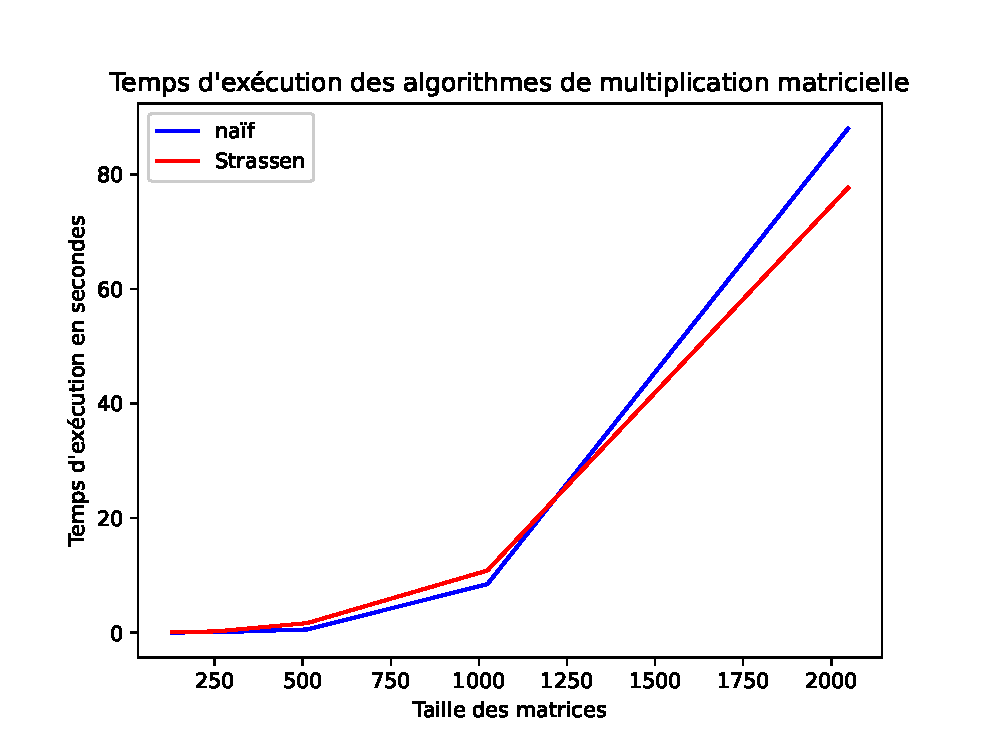
\includegraphics[width=120px]{\SPATH/strassen.eps}
			\end{center}
		}
	\end{exampleblock}
\end{frame}

\makess{Rappel : mémoïsation}
\begin{frame}{\Ctitle}{\stitle}
	\begin{exampleblock}{Exemple}
		\begin{enumerate}
			\item<1-> Ecrire une fonction récursive \textit{naïve} en Ocaml qui prend en argument un entier $n$ et renvoie le $n$ième terme de la suite de Fibonacci définie par :
				$\left\{ \begin{array}{lll}
						f_0   & = & 1,                                                  \\
						f_1   & = & 1,                                                  \\
						f_{n} & = & f_{n-1}+f_{n-2} \mathrm{\ \ pour\ tout\ \ } n\geq2.\end{array} \right.$
					\onslide<2->{\inputpartOCaml{\SPATH/fibo.ml}{}{}{1}{2}}
			\item<3-> Tracer le graphe des appels récursifs de cette fonction pour $n=5$
			\item<4-> Commenter
		\end{enumerate}
	\end{exampleblock}
\end{frame}



\begin{frame}{\Ctitle}{\stitle}
	\begin{exampleblock}{Exemple}
		\begin{center}
			\psset{levelsep=1cm,treesep=0.2cm,linecolor=OliveGreen,linewidth=0.6pt}
			\pstree{\Toval{\tiny \tt fibo(5)}}{
				\pstree{\Toval{\tiny \tt fibo(4)}}{
					\pstree{\Toval{\tiny \tt  fibo(3)}}{
						\pstree{\Toval{\textcolor{BrickRed}{\tt \tiny fibo(2)}}}{\Toval{\tt \tiny fibo(1)} \Toval{\tiny \tt  fibo(0)}}
						\Toval{\tiny \tt  fibo(1)}}
					\pstree{\Toval{\textcolor{BrickRed}{\tt \tiny fibo(2)}}}{\Toval{\tiny  \tt fibo(1)} \Toval{\tiny \tt  fibo(0)}}
				}
				\pstree{\Toval{\tiny \tt fibo(3)}}{
					\pstree{\Toval{\textcolor{BrickRed}{\tt \tiny fibo(2)}}}{\Toval{\tiny \tt  fibo(1)} \Toval{\tiny \tt  fibo(0)}}
					\Toval{\tiny \tt  fibo(1)}}
			}
		\end{center}
		\onslide<2-> Les mêmes appels récursifs apparaissent dans plusieurs branche, on dit qu'il y a \textcolor{blue}{\textit{chevauchement des appels récursifs}}.
		\onslide<3-> (On peut montrer que le nombre d'appels récursifs $a_n$ pour calculer $f_n$ est $a_n = 2\,f_n -1$ et donc la complexité est exponentielle)
	\end{exampleblock}
\end{frame}



\begin{frame}{\Ctitle}{\stitle}
	\begin{alertblock}{Mémoïsation}
		\begin{itemize}
			\item<1-> La \textcolor{blue}{mémoïsation} consiste à stocker dans une structure de données les valeurs renvoyées par une fonction afin de ne pas les recalculer lors des appels identiques suivant.\\
			\item<2-> Les tableaux associatifs dont les clés sont les arguments de la fonction et les valeurs les résultats correspondant sont des structures de données adaptées à ce stockage car on teste l'appartenance et on retrouve une valeur efficacement.
			\item<3-> On rappelle qu'un tableau associatif peut-être implémenté de façon efficace par :
			\begin{itemize}
				\item une table de hachage 
				\item un arbre binaire de recherche lorsque les clés sont ordonnées.
			\end{itemize}
		\end{itemize}
	\end{alertblock}
\end{frame}


\makess{Programmation dynamique : exemple introductif}
\begin{frame}{\Ctitle}{\stitle}
	\begin{exampleblock}{Position du problème}
		\onslide<1->{\small On considère une barre de métal de longueur entière 12 et pouvant être découpée en morceaux de longueurs entières ayant chacun un prix comme indiqué ci-dessous :
			\begin{center}
				\begin{tabular}{|l|p{0.2cm}|p{0.2cm}|p{0.2cm}|p{0.2cm}|p{0.2cm}|p{0.2cm}|p{0.2cm}|p{0.2cm}|p{0.2cm}|p{0.2cm}|p{0.2cm}|p{0.2cm}|}
					\hline
					longueur ($i$) & 1 & 2 & 3 & 4 & 5  & 6  & 7  & 8  & 9  & 10 & 11 & 12 \\
					\hline
					prix     ($p_i$)& 2 & 4 & 7 & 8 & 12 & 14 & 18 & 23 & 24 & 25 & 26 & 31 \\
					\hline
				\end{tabular}
			\end{center}}
		\onslide<2->{\small Le prix de vente des différents morceaux varie donc suivant la découpe utilisée, par exemples :
			la découpe $(2, 4, 6)$ a un prix de vente de $4+8+14=26$, tandis que la découpe $(7, 5)$ a un prix de vente de $18+12=30$\\}
		\onslide<3->\textcolor{blue}{\small Le but du problème est de trouver la valeur maximale des découpes possibles.\\}
		\onslide<4->{\small On note $N$ la longueur de la barre, $(v_i)_{1\leq i \leq N}$, la valeur maximale de la découpe d'une barre de taille $i$ et $(p_i)_{1 \leq i \leq N}$ le prix d'un morceaux de longueur $i$.}
		\begin{enumerate}
			\item<5-> {\small Donner les valeurs de $v_0$, $v_1$, $v_2$ et $v_3$.}
			\item<6-> {\small Etablir une relation de récurrence liant les $(v_i)_{0\leq i \leq N}$.}
			\item<7-> {\small En déduire une fonction  récursive en C calculant la valeur de la découpe maximale.}
			\item<8-> {\small Vérifier qu'on se trouve dans une situation de chevauchement des appels récursifs et proposer une nouvelle version de votre fonction utilisant la mémoïsation.}
			\item<9-> {\small Etudier les complexités des deux versions.}
		\end{enumerate}
	\end{exampleblock}
\end{frame}

\begin{frame}{\Ctitle}{\stitle}
	\begin{exampleblock}{Résolution}
		\begin{enumerate}
			\item<1-> \textcolor{OliveGreen}{\small $v_0=0$, $v_1=2$, $v_2 = 4$ et $v_3 = 7$ }
			\item<2-> \textcolor{OliveGreen}{\small En supposant qu'on connaisse les valeurs maximales de découpe pour \textit{toutes} les tailles inférieures à $n$, la découpe maximale pour la taille $n$ s'en déduit en prenant le maximum parmi les découpes maximales d'une barre de longueur $n-k \leq n-1$  et du prix d'un morceau de taille $k$, c'est à dire :
					$v_n = \max\left\{ v_{n-k} + p_{k},  1 \leq k \leq n\right\}$}
			\item<3-> \textcolor{OliveGreen}{\small Implémentation en C:}
				\inputpartC{\SPATH/barre.c}{}{\footnotesize}{19}{28}
		\end{enumerate}
	\end{exampleblock}
\end{frame}


\begin{frame}{\Ctitle}{\stitle}
	\begin{exampleblock}{Résolution}
		\begin{enumerate}
			\addtocounter{enumi}{3}
			\item Pour calculer $v_5$, on doit calculer $v_4, v_3, \dots v_0$. Mais l'appel à $v_4$ demande aussi le calcul de $v_3, v_2, \dots v_0$. On se trouve donc bien dans le cas d'un chevauchement d'appels récursifs. \\
			\medskip
			On peut proposer la version avec memoisation suivante :
			\inputpartC{\SPATH/barre.c}{}{\footnotesize}{30}{40}
		\end{enumerate}
	\end{exampleblock}
\end{frame}

\begin{frame}{\Ctitle}{\stitle}
	\begin{exampleblock}{Résolution}
		\begin{enumerate}
			\addtocounter{enumi}{4}
			\item On peut construire l'arbre des appels récursifs pour $n=5$ :\\
			\onslide<2->{\begin{center}
			\psset{levelsep=1cm,treesep=0.2cm,linecolor=OliveGreen,linewidth=0.6pt}
			\pstree{\TCircle{$v_5$}}{
				\TCircle{$v_1$}
				\pstree{\TCircle{$v_2$}}{
					\TCircle{$v_1$}}
				\pstree{\TCircle{$v_3$}}{
						\TCircle{$v_1$}
						\pstree{\TCircle{$v_2$}}{
						\TCircle{$v_1$}}
						}
				\pstree{\TCircle{$v_4$}}{
					\TCircle{$v_1$}
					\pstree{\TCircle{$v_2$}}{
					\TCircle{$v_1$}}
					\pstree{\TCircle{$v_3$}}{
						\TCircle{$v_1$}
						\pstree{\TCircle{$v_2$}}{
						\TCircle{$v_1$}}
						}
				}
			}
			\end{center}}
			\onslide<3->{En notant $a_n$ le nombre d'appels pour calculer $v_n$, on a $\displaystyle{a_n = 1 + \sum_{k=0}^{n-1} a_k}$.}
			\onslide<4->{On obtient $a_n = 2^n$ et donc la complexité est au moins quadratique !}
		\end{enumerate}
	\end{exampleblock}
\end{frame}

\begin{frame}{\Ctitle}{\stitle}
	\begin{exampleblock}{Résolution}
		\begin{enumerate}
			\addtocounter{enumi}{4}
			\item Dans le cas de la mémoïsation, les appels récursifs déjà calculés sont obtenus directement, ce qui donne l'arbre d'appel suivant :
			\onslide<2->{\begin{center}
				\psset{levelsep=1cm,treesep=0.2cm,linecolor=OliveGreen,linewidth=0.6pt}
				\pstree{\TCircle{$v_5$}}{
					\TCircle{$v_1$}
					\pstree{\TCircle{$v_2$}}{
						\TCircle{$v_1$}}
					\pstree{\TCircle{$v_3$}}{
							\TCircle{$v_1$}
							\TCircle{$v_2$}
							}
					\pstree{\TCircle{$v_4$}}{
						\TCircle{$v_1$}
						\TCircle{$v_2$}
						\TCircle{$v_3$}
						}
					}
				\end{center}}
				\onslide<3->{En notant $b_n$ le nombre d'appels pour calculer $v_n$, on a $\displaystyle{b_n = \sum_{k=0}^{n-1} k}$.}
			\onslide<4->{La complexité est donc quadratique.}
		\end{enumerate}
	\end{exampleblock}
\end{frame}

\begin{frame}{\Ctitle}{\stitle}
	\begin{exampleblock}{Calcul de bas en haut (\textit{bottom up})}
		\onslide<1->{\small La mémoïsation construit la solution de façon "descendante", on lance les appels récursif sur les plus grandes valeurs de taille de la barre. Une autre stratégie dite \textcolor{blue}{ascendante} ou \textcolor{blue}{de bas en haut (\textit{bottom up})} consiste à construire la solution en partant des instances les plus petites du problème.\\}
		\onslide<2->{\small Pour la découpe de la barre on part donc des valeurs connues $v_0$ et $v_1$ et on construit $v_2$ puis $v_3$, en utilisant la relation de récurrence $v_n = \max\left\{ v_{n-k} + p_{k},  1 \leq k \leq n\right\}$}\\
		\onslide<3->{\small Ce qui se traduit  par une solution \textcolor{blue}{itérative} :}
		\onslide<4->{\inputpartC{\SPATH/barre.c}{}{\footnotesize}{43}{52}}
	\end{exampleblock}
\end{frame}

\begin{frame}{\Ctitle}{\stitle}
	\begin{exampleblock}{Construction d'une solution}
		On a pour le moment déterminé la valeur maximale de la découpe, mais pas la découpe elle-même. D'autre part, plusieurs découpes différentes peuvent avoir cette même valeur maximale. Pour rechercher \textit{une} découpe de valeur maximale, on peut par exemple :
		\begin{itemize}
			\item<1-> construire le tableau $(v_k)_{0\leq k \leq\N}$  et l'utiliser afin d'en déduire la découpe. \\
				\onslide<2->{\textcolor{gray}{\small Par exemple, si $v_{12} = v_8 + p_4$, cela signifie que pour avoir la valeur maximale de la découpe d'une barre de taille 12, une possibilité est d'utiliser une découpe  maximale d'une barre de taille 8 et un morceau de taille 4. En remontant ainsi de proche en proche, on obtient une découpe maximale possible}}
			\item<3-> Modifier notre fonction afin qu'elle renvoie la découpe maximale et non pas la valeur de cette découpe. \\
		\end{itemize}
		\onslide<4->{Ces deux possibilités seront abordées en TP.}
	\end{exampleblock}
\end{frame}


\makess{Programmation dynamique}
\begin{frame}{\Ctitle}{\stitle}
	\begin{alertblock}{Principes généraux}
		La programmation dynamique s'applique généralement à la résolution d'un problème d'optimisation vérifiant les conditions suivantes :
		\begin{enumerate}
			\item<2-> \textcolor{blue}{Sous structure optimale} : ce problème peut-être résolu à partir de problèmes similaires mais plus petits \\
				\onslide<3->\textcolor{gray}{\small La découpe maximale d'une barre de taille $N$ s'obtient comme découpe maximale  d'une barre de taille strictement inférieure $k$ et d'un morceau de taille $N-k$.}
				\item<4->\textcolor{blue}{Chevauchement de sous problème} : une solution récursive produit des appels identiques. Pour pallier ce problème, on utilise la mémoïsation dans les solutions récursives ou une solution de bas en haut itérative.\\
				\onslide<5->\textcolor{gray}{\small Pour rechercher la découpe maximale d'un barre de taille 5, on est amené à chercher celle d'une barre de taille 4,3,2,1. Et pour chercher celle d'une barre de taille 4, on fera de nouveau appel à celle d'une barre de taille 3,2,1 ...}
		\end{enumerate}
		\onslide<6->{\textcolor{BrickRed}{\small \important} L'étape cruciale est de déterminer les relations de récurrence entre les différentes instances du problème.}
	\end{alertblock}
\end{frame}

\begin{frame}{\Ctitle}{\stitle}
	\begin{exampleblock}{Sous structure optimale : contre-exemples}
	On donne ici deux exemples de problèmes n'ayant \textit{pas} la propriété de \textcolor{blue}{sous structure optimale} :
		\begin{itemize}
			\item<2-> Nombre minimal de multiplications dans le calcul de $a^n$\\
			\onslide<3->\textcolor{gray}{\small Par exemple le calcul optimal de $a^{15}$ demande 5 multiplications : $a^{15} = a^3 \times \left((a^3)^2\right)^2$ \\ $a^6$ doit donc être donc calculé en utilisant le calcul de $a^3$ au lieu de par exemple $a^6 = (a^2)^3$ qui demande aussi 3 multiplications. C'est à dire qu'on peut avoir trouvé une solution optimale $n=6$ mais qui n'intervient \textit{pas} dans le calcul pour $n=15$.}
			\item<4-> Recherche du plus long chemin élémentaire dans un graphe\\
			\onslide<5->{
			\begin{tabularx}{\linewidth}{p{2.5cm}X}
				\begin{tabular}{lr}
					\circlenode[linecolor=gray]{a}{\textcolor{gray}{$a$}} \hspace{1cm} & \circlenode[linecolor=gray]{b}{\textcolor{gray}{$b$}} \vspace{1cm}\\
					\multicolumn{2}{c}{\circlenode[linecolor=gray]{c}{\textcolor{gray}{$c$}}}\\
				\end{tabular} 
				\ncarc[linecolor=gray]{->}{a}{b} \ncarc[linecolor=gray]{->}{a}{c} \ncarc[linecolor=gray]{->}{b}{a} \ncarc[linecolor=gray]{->}{b}{c} \ncarc[linecolor=gray]{->}{c}{a} \ncarc[linecolor=gray]{->}{c}{b}
				& \vspace{-1cm}
				\textcolor{gray}{\small Dans le graphe ci-contre, le plus long chemin élémentaire de $a$ vers $c$ est $a \rightarrow b \rightarrow c$ et son sous-chemin $a \rightarrow b$ n'est pas une la solution du sous problème consistant à rechercher le plus long chemin élémentaire de $a$ vers $b$. Et de même pour son sous chemin $b \rightarrow c$.}
			\end{tabularx}}
		\end{itemize}
	\end{exampleblock}
\end{frame}



\makess{Exemple résolu : plus longue sous séquence commune}
\begin{frame}{\Ctitle}{\stitle}
	\begin{exampleblock}{Position du problème}
		On considère deux chaines de caractères $u$ et $v$ de longueurs respectives $n$ et $m$. On cherche à déterminer la longueur de leur \textcolor{blue}{p}lus \textcolor{blue}{l}ongue \textcolor{blue}{s}ous \textcolor{blue}{s}équence \textcolor{blue}{c}ommune (\textcolor{blue}{\sc plssc}), c'est à dire la chaine $w$ telle que :
		\begin{itemize}
			\item<2-> $w$ est une sous séquence (c'est à dire une suite extraite) de $u$,
			\item<3-> $w$ est une sous séquence de $w$,
			\item<4-> $w$ est de longueur maximale.
		\end{itemize}
		\onslide<5->{Par exemple,  $u$="{\sc programmation}" et $v$="{\sc dynamique}" ont comme sous séquence commune "{\sc ami}" (et c'est la plus longue)}
		\begin{itemize}
			\item<6-> {\sc progr\textcolor{BrickRed}{a}m\textcolor{BrickRed}{m}at\textcolor{BrickRed}{i}on}
			\item<7-> {\sc dyn\textcolor{BrickRed}{ami}que}
		\end{itemize}
		\onslide<8->{Donc ici, la longueur de la {\sc plssc} est 3.}
	\end{exampleblock}
\end{frame}

\begin{frame}{\Ctitle}{\stitle}
	\begin{exampleblock}{Résolution}
		On cherche les relations de récurrence entre des instances du sous-problème. Pour cela on note $u_i$ ($0\leq i \leq n$) la chaine composée des $i$ premiers caractères de $u$, et $v_j$ ($0\leq j \leq m$) celle composée des $j$ premiers caractères de $v$. Et on note $\mathrm{lplssc}(u_i,v_j)$ la longueur de la {\sc plssc} de $u_i$ et de $v_j$.
		\begin{itemize}
			\item<2->{Si $u[i] = v[j]$ alors, quelle est la relation entre $\mathrm{lplssc}(u_i,v_j)$ et $\mathrm{lplssc}(u_{i-1},v_{j-1})$ ? \\}
			\onslide<5->{\textcolor{OliveGreen}{$\mathrm{lplssc}(u_i,v_j) = 1 + \mathrm{lplssc}(u_{i-1},v_{j-1})$}}
			\item<3->{Sinon, exprimer $\mathrm{plssc}(u_i,v_j)$ en fonction de  $\mathrm{plssc}(u_{i},v_{j-1})$  et $\mathrm{plssc}(u_{i-1},v_j)$}
			\onslide<6->{\textcolor{OliveGreen}{$\mathrm{lplssc}(u_i,v_j) = \max\left(\mathrm{lplssc}(u_{i},v_{j-1}) ,\mathrm{lplssc}(u_{i-1},v_{j})\right)$}}
			\item<4->{Déterminer les cas de base (ceux où $u$ et $v$ sont des chaines vides notés $\epsilon$):\\}
			\onslide<7->{\textcolor{OliveGreen}{$\mathrm{lplssc}(u_{i},\epsilon) = 0$} \\
				\textcolor{OliveGreen}{$\mathrm{lplssc}(\epsilon,v_j) = 0$} }
		\end{itemize}
	\end{exampleblock}
\end{frame}


\begin{frame}{\Ctitle}{\stitle}
	\begin{exampleblock}{Implémentation en OCaml}
		On doit donc écrire une fonction {\tt lplssc string -> string -> int} qui prend en argument deux chaines de caractères {\tt u} et {\tt v} et renvoie la longueur de leur plus longue sous séquence commune.\\
		\onslide<2->{\textcolor{OliveGreen}{\small \aide} Comme on travaille récursivement sur la longueur des prefixes on pourra écrire une fonction auxiliaire {\tt aux  string -> string -> int -> int -> int} qui prend deux entiers supplémentaires en arguments : les longueurs de chacune des deux chaines}
		\onslide<3->{\inputpartOCaml{\SPATH/plssc.ml}{}{}{1}{7}}
	\end{exampleblock}
\end{frame}

\begin{frame}{\Ctitle}{\stitle}
	\begin{exampleblock}{Mémoïsation}
		{\small Modifier la fonction précédente afin de mémoriser les résultats déjà calculés. On pourra utiliser une matrice {\tt memo} crée en OCaml avec \mintinline{Ocaml}{let memo = Array.make_matrix (n+1) (m+1) (-1)}\\ La valeur initiale $-1$ indiquant que la {\sc lplssc} de $u_i$ et $v_j$ n'a pas encore été calculée.}
		\onslide<3->{\inputpartOCaml{\SPATH/plssc.ml}{}{\footnotesize}{10}{22}}
	\end{exampleblock}
\end{frame}

\begin{frame}{\Ctitle}{\stitle}
	\begin{exampleblock}{Version itérative}
		\onslide<2->{\inputpartOCaml{\SPATH/plssc.ml}{}{\footnotesize}{37}{54}}
	\end{exampleblock}
\end{frame}

\begin{frame}{\Ctitle}{\stitle}
	\begin{exampleblock}{Reconstruction de la solution}
		{\small La matrice obtenue pour les mots : {\sc imperial} et {\sc empire} est : \\}
		\quad \quad \begin{tabular}{|>{\tt}c|>{\tt}c|>{\tt}c|>{\tt}c|>{\tt}c|>{\tt}c|>{\tt}c|>{\tt}c|}
			
			\cline{2-8}
		\multicolumn{1}{c|}{}	& \textcolor{blue}{$\epsilon$}  & \textcolor{blue}{E}  &\alt<17->{\textcolor{red}{M}}{\textcolor{blue}{M}} &\alt<15->{\textcolor{red}{P}}{\textcolor{blue}{P}} &\alt<11->{\textcolor{red}{I}}{\textcolor{blue}{I}} &\textcolor{blue}{R} & \textcolor{blue}{E} \\
			\hline
			\textcolor{blue}{$\epsilon$}	& 0 &0 &0 &0 &0 &0 &0 \\ 
		\textcolor{blue}{I}	& 0 & \alt<18->{\textcolor{red}{0}}{0} &0 &0 &1 &1 &1 \\ 
		\alt<17->{\textcolor{red}{M}}{\textcolor{blue}{M}}	& 0 &0 &\alt<16->{\textcolor{red}{\underline 1}}{1} &1 &1 &1 &1 \\ 
		\alt<15->{\textcolor{red}{P}}{\textcolor{blue}{P}}	& 0 &0 & 1 &\alt<14->{\textcolor{red}{\underline 2}}{2} &2 &2 &2 \\ 
		\textcolor{blue}{E}	& 0 &1 &1 &\alt<13->{\textcolor{red}{2}}{2} &2 &2 &3 \\ 
		\textcolor{blue}{R}	& 0 &1 &1 &\alt<12->{\textcolor{red}{2}}{2} &2 &3 &3 \\ 
		\alt<11->{\textcolor{red}{I}}{\textcolor{blue}{I}}	& 0 &1 &1 &2 &\alt<10->{\textcolor{red}{\underline 3}}{3} &3 &3 \\ 
		\textcolor{blue}{A}	& 0 &1 &1 &2 &\alt<9->{\textcolor{red}{3}}{3} &3 &3 \\ 
		\textcolor{blue}{L}	& 0 &1 &1 &2 &\alt<8->{\textcolor{red}{3}}{3} &\alt<7->{\textcolor{red}{3}}{3} &\alt<6->{\textcolor{red}{3}}{3} \\
		\hline
		\end{tabular}\\
	\onslide<2->{\small On peut utiliser ce résultat pour construire la {\sc plssc} :}
	\begin{itemize}
		\item<3-> {\small on part de la dernière case en bas et à droite}
		\item<4-> {\small si les lettres sur la ligne et la colonne sont identiques on ajoute à la {\sc plssc} et on remonte en diagonale}
		\item<5-> {\small sinon on va à gauche ou en haut suivant la case qui a plus grande valeur}
	\end{itemize}
	\end{exampleblock}
\end{frame}


\begin{frame}{\Ctitle}{\stitle}
	\begin{exampleblock}{Reconstruction de la solution}
		\onslide<2->{\inputpartOCaml{\SPATH/plssc.ml}{}{\footnotesize}{59}{74}}
	\end{exampleblock}
\end{frame}


\makess{Exemple résolu : rendu de monnaie}
\begin{frame}{\Ctitle}{\stitle}
	\begin{exampleblock}{Position du problème}
		On dispose d'un \textit{système monétaire} c'est à dire d'un ensemble de valeurs possibles pour les pièces et les billets. Le problème du rendu de monnaie consiste à déterminer le nombre minimal de pièces à utiliser pour former une somme donnée. \\
		\onslide<2->{Par exemple si le système monétaire est $\{ 1, 3, 4, 5 \}$ et la somme 7,}
		\onslide<3->{alors on peut utiliser au minimum 2 pièces ($4+3$).}\\
		\onslide<5->{\textcolor{blue}{\small \rappel \; Rappel : }{\textcolor{gray}{ l'algorithme glouton qui consiste à rendre à tout moment la pièce de plus forte valeur possible ne fournit pas toujours la solution optimale. Ici, on obtiendrait $5, 1, 1$ et donc 3 pièces.}}}
		\begin{enumerate}
			\item<6-> Ecrire une relation de récurrence entre les différentes instances du problème en donnant les solutions des cas de base.
			\item<7-> Ecrire un programme en C permettant de répondre au problème.
			\item<8-> Construire la liste effective des pièces à rendre.
		\end{enumerate}
	\end{exampleblock}
\end{frame}


\begin{frame}{\Ctitle}{\stitle}
	\begin{exampleblock}{Résolution}
		\begin{enumerate}
			\item<2->\textcolor{black}{On note} :
			\begin{itemize}
				\item<3->\textcolor{black}{$s$ la somme à rendre,}
				\item<4->\textcolor{black}{$(p_i)_{1 \leq i \leq n}$ les valeurs des pièces rangées dans l'ordre \textit{croissant}}
				\item<5->\textcolor{black}{$m(s,k)$ le nombre minimal de pièce pour rendre la somme~$s$ en utilisant les pièces $(p_i)_{1 \leq i \leq k}$}
			\end{itemize}
			\onslide<6->\textcolor{black}{Avec ces notations, on doit donc trouver $m(s,n)$ et on dispose des relations suivantes :} \\
			\onslide<7->{\textcolor{black}{$\left\{ \begin{array}{lll}
							m(0,k)   & = & 0 \text{ pour tout } 1\leq k \leq n,                         \\
							m(s,0) & = & +\infty \text{ pour tout } s \in \N^*,                                                     \\
							m(s,k)   & = & m(s,k-1)    \text{ si }  s<p_k,                              \\
							m(s,k)   & = & \min\left\{ 1 + m(s-p_k,k), m(s,k-1) \text{  }\right\} \text{ sinon.}\end{array} \right.$}\medskip \\}
		\end{enumerate}
	\end{exampleblock}
\end{frame}

\begin{frame}{\Ctitle}{\stitle}
	\begin{exampleblock}{Résolution}
		\begin{enumerate}
			\addtocounter{enumi}{1}
			\item Programme en C 
			\onslide<2->{\inputpartC{\SPATH/rendu.c}{}{}{7}{14}}
			\onslide<3->{Comme pour la {\sc plssc}, on peut écrire une solution itérative ou une solution utilisant la mémoïsation.}
		\end{enumerate}
	\end{exampleblock}
\end{frame}

\begin{frame}{\Ctitle}{\stitle}
	\begin{exampleblock}{Reconstruction de la solution}
		\begin{enumerate}
			\addtocounter{enumi}{2}
			\item On construit une solution effective à partir des valeurs de la matrice~$m(s,k)$ \\
			      \renewcommand{\arraystretch}{1.3}
			      \begin{tabular}{|c|c|c|c|c|c|c|}
				      \cline{2-6}
					  \multicolumn{1}{c|}{} & \textcolor{blue}{0} &  \textcolor{blue}{1}  {\tiny ($\scriptstyle p_1=1$)}  & \textcolor{blue}{2} {\tiny ($\scriptstyle p_2=3$)} & \textcolor{blue}{3} {\tiny ($\scriptstyle p_3=4$)}& \textcolor{blue}{4} {\tiny ($\scriptstyle p_4=5$)} \\
					  \hline
				      	\textcolor{blue}{0}& 0 & 0 & 0 & 0 & 0 \\ 
						\textcolor{blue}{1}& $\infty$ & 1 & 1 & 1 & 1 \\ 
						\textcolor{blue}{2}& $\infty$ & 2 & 2 & 2 & \alt<2->{\circlenode[linecolor=blue]{r1}{\textcolor{blue}{2}}}{2} \\ 
						\textcolor{blue}{3}& $\infty$ & 3 & 1 & 1 & 1 \\ 
						\textcolor{blue}{4}& $\infty$ & 4 & 2 & 1 & 1 \\ 
						\textcolor{blue}{5}& $\infty$ & 5 & 3 & 2 & 1 \\ 
						\textcolor{blue}{6}& $\infty$ & 6 & 2 & 2 & 2 \\ 
						\textcolor{blue}{7}& $\infty$ & 7 & 3 & \alt<4->{\circlenode[linecolor=blue]{r0}{\textcolor{blue}{2}}}{2} & \circlenode[linecolor=red]{r2}{\textcolor{red}{2}} \\ 
					\hline
			      \end{tabular}
				  \onslide<3->{\ncbar[angleA=0, angleB=0, linestyle=dashed, linecolor=red]{->}{r2}{r1} \nbput{$\boxed{p_4}$}}
				  \onslide<4->{\ncline[linestyle=dashed, linecolor=red]{->}{r2}{r0}}
		\end{enumerate}
	\end{exampleblock}
\end{frame}


\end{document}